\documentclass{article}
\usepackage{geometry}
\usepackage{hyperref}
\usepackage{lipsum}
\title{\vspace{180pt}Sorting on FPGAs using Merge Trees}
\vspace{-10pt}
\author{\vspace{-5pt} Nikola Samardzic\\ \href{mailto:nikola.s@ucla.edu}{nikola.s@ucla.edu}}
\date{}
\usepackage{mathtools}
\usepackage{mathptmx}
\usepackage{amsfonts}
\usepackage{graphicx}
\usepackage{subcaption}
\usepackage[dvipsnames]{xcolor}
\usepackage[utf8]{inputenc}
\usepackage[english]{babel}
\usepackage{wrapfig}
\usepackage{fancyhdr}
\usepackage{float}
\usepackage{multicol}
\usepackage{algorithmic}
\usepackage{enumitem}
\setlist[enumerate]{itemsep=0mm}
\newcommand{\Poly}{\textsc{P}}
\newcommand{\SAT}{\textsc{SAT}}
\newcommand{\NP}{\textsc{NP}}
\newcommand{\RP}{\textspc{RP}}
\newcommand{\BPP}{\textsc{BPP}}
\newcommand{\EXP}{\textsc{EXP}}
\newcommand{\NEXP}{\textsc{NEXP}}
\newcommand{\PSPACE}{\textsc{PSPACE}}
\newcommand{\PH}{\textsc{PH}}
\linespread{1.5}

\usepackage{listings}
\usepackage{color}

\definecolor{dkgreen}{rgb}{0,0.6,0}
\definecolor{gray}{rgb}{0.5,0.5,0.5}
\definecolor{mauve}{rgb}{0.58,0,0.82}

\lstset{frame=tb,
  language=Java,
  aboveskip=3mm,
  belowskip=3mm,
  showstringspaces=false,
  columns=flexible,
  basicstyle={\small\ttfamily},
  numbers=none,
  numberstyle=\tiny\color{gray},
  keywordstyle=\color{blue},
  commentstyle=\color{dkgreen},
  stringstyle=\color{mauve},
  breaklines=true,
  breakatwhitespace=true,
  tabsize=3
}

\usepackage{tcolorbox}
\usepackage{amsmath}
\usepackage{amssymb}
\usepackage{amsthm}
\newtheorem{lemma}{Lemma}
\newtheorem{claim}{Claim}
\newtheorem{remark}{Remark}
\newtheorem{problem}{Problem}
\pagestyle{fancy}
\fancyhf{}
\fancyhead[RE,LO]{Spring 2019, CS 199 Final Report}
\fancyhead[LE,RO]{Nikola Samardzic}
\setcounter{problem}{25}
\usepackage{setspace}
\singlespacing
\begin{document}
\clearpage\maketitle
\thispagestyle{empty}
\newpage
\tableofcontents
\newpage
\section{Abstract}
\textit{Hardware Mergers} can be used to implement sorting algorithms on Field-Programmable Gate Arrays (FPGAs) by inductively merging elements as in the Merge Sort algorithm.\cite{fccm17}\cite{fccm18} These Hardware Mergers have also been laid out onto the FPGA in a complete binary tree pattern (called a \textit{Hardware Merge Tree}) which further enhances performance of the sorting procedure by merging many input arrays at once.\cite{camb} In \cite{terabyte} the authors recognize the need for using different Merger Trees when sorting on different levels of the memory hierarchy (On-Chip, DRAM, or Flash). Nonetheless, their choice of Merge Trees at each level of the hierarchy is rather ad hoc and there is no rigorous analysis to justify their design choices.

In this work, we develop a comprehensive analytical model that takes into consideration the off-chip memory bandwidth and the amount of on-chip resources to optimize the overall sorting latency. Further, we develop methods for implementing a wider range of Merge Trees as well as a general DRAM access pattern and data loading model that operates at peak DRAM bandwidth without affecting the throughput of the Merge Tree. As all signals in our Merge Tree are local to the tree nodes (Hardware Mergers), the design can be scaled to future improvements in FPGA resource availability as well as to a network of many interconnected FPGAs, without impact to the Merge Tree throughput.

We present the only end-to-end sorting design on FPGAs aside from the design in \cite{terabyte}. Cycle-accurate simulations of our design report that it outperforms in total sorting time the implementation in \cite{terabyte} on the same hardware setup by 3.1x. Our cycle-accurate software simulations which account for DRAM random access and sequential access trade-offs demonstrates that our end-to-end design has total sorting time within 90\% of the predictions of our model.

\section{Introduction}

% \textcolor{blue}{\textbf{[IMPROTANCE OF DOMAIN-SPECIFIC DEVICES]}}

Growing computational needs can no longer be met by appropriately scaling the number of transistors on chip due to unsustainable costs and physical limitations.\cite{nyt_article} \cite{end_of_moore} One popular way of addressing this problem is by developing customizable hardware devices that are used as domain-specific components of a larger computer system. These domain-specific devices can then be reconfigured to efficiently and quickly perform a specific computation (usually this computation is the bottleneck of the computer system). This approach allows us to bypass the computational bottlenecks inherent in modern Central Processing Units (CPU). Namely, CPUs and their associated Instruction Set Architectures (ISAs) are good at meeting general computing needs with minimal hardware requirements, but may be inadequate for large-scale, repetitive, and compute-intensive tasks.

% \textcolor{blue}{\textbf{[APPLICATIONS OF LARGE-SCALE SORTING]}}

Sorting is an important part of many data center applications. For example, in \textit{MapReduce} keys coming out of the mapping stage must be sorted prior to being fed into the reduce stage. \cite{mapreduce} More generally, large-scale sorting is needed to run social networks, IoT devices, and relational database. In relational database management systems specifically, the \textit{merge join} algorithm has been in focus of many research groups due to its relative importance and high computational overhead.\cite{microsoft_merge_join}\cite{eth_merge_join}

\subsection{Current State-of-the-Art Results}
% \textcolor{blue}{\textbf{[LIST STATE-OF-THE-ART RESULTS]}} 

The website \hyperref[sortbenchmark.org]{sortbenchmark.org} hosts a set of benchmarks as well as a list of best performers for each category. The benchmarks were originally created by Prof. Jim Gray. The benchmarks are:
\begin{itemize}[noitemsep,topsep=0pt,parsep=0pt,partopsep=0pt]
\item \textit{Gray}. Measures sort rate (terabytes / minute) achieved while sorting a very large amount of data (at least $100$ TB).
\item \textit{Cloud}. Measures cost for sorting a very large amount of data on the public cloud. (currently $100$ TB) \cite{cloudsort}
\item \textit{Minute}. Measures amount of data that can be sorted in one minute or less. \cite{alphasort}
\item \textit{Joule}. Measures energy required to sort $10^8$, $10^9$, $10^{10}$, or $10^{12}$ records ($10$ GB, $100$ GB, $1$ TB, $100$ TB). \cite{joulesort}
\end{itemize}

The \textit{Indy} benchmark uses the record size of 100 bytes with the first 10 bytes being a random key. For the \textit{Daytona} benchmark, the implementation must be general purpose, sorting any width key-value pairs. The current record holders are listed in Table~\ref{tab:benchmark}.

\begin{table}[]
\renewcommand{\arraystretch}{2}
\centering
\begin{tabular}{|c|c|c|}
\hline
 &\textbf{Daytona}  &\textbf{Indy}  \\
 \hline
\textbf{Gray} & \renewcommand{\arraystretch}{1}\begin{tabular}{c}Tencent Sort \cite{tencent}\\ 44.8 TB/min \end{tabular} &\renewcommand{\arraystretch}{1}\begin{tabular}{c}Tencent Sort \\ 60.7 TB/min \end{tabular}\\
\hline
\textbf{Cloud} & \renewcommand{\arraystretch}{1}\begin{tabular}{c}NADSort \cite{nadsort} \\ \$1.44/TB \end{tabular}& \renewcommand{\arraystretch}{1}\begin{tabular}{c}NADSort \\ \$1.44/TB \end{tabular}  \\
\hline
\textbf{Minute} & \renewcommand{\arraystretch}{1}\begin{tabular}{c}Tencent Sort \\ 37 TB \end{tabular} & \renewcommand{\arraystretch}{1}\begin{tabular}{c}Tencent Sort \\ 55 TB \end{tabular} \\
\hline
\textbf{Joule} ($10^{10}$ records) &\renewcommand{\arraystretch}{1}\begin{tabular}{c}NTOSort \cite{ntosort} \\ 59,444 records/Joule \end{tabular} &\renewcommand{\arraystretch}{1}\begin{tabular}{c}NTOSort\\ 59,444 records/Joule \end{tabular} \\
\hline
\end{tabular}
\caption{sortbenchmark.org record holders.}
\label{tab:benchmark}
\end{table}

We believe it would be achievable to break the JouleSort record with our implementation. In fact, the authors in \cite{terabyte} -- on which our design is based -- argue that their design has double the power performance of NTOSort, and that an optimization of their approach should reach 200,000 records/Joule.


\subsection{Survey of Previous Work}

% \textcolor{blue}{\textbf{[LIST PREVIOUS WORK ON CPU , GPU, FPGA, ASIC SORTING]}}

Many modern sorting algorithms are entirely implemented on commodity CPUs. These algorithms usually take advantage of Intel's Streaming Single-Instruction Multiple-Data (SIMD) instructions.\cite{SIMD}\cite{cache-friendly}\cite{radix} Another popular approach includes using General Purpose Graphics Processing Units (GPGPUs). \cite{manycore}\cite{gputera}\cite{gpu_radix} We suggest \cite{gpu_survey} as a good introductory survey paper for sorting on GPUs. There is also research in using Application Specific Integrated Circuits (ASICs). \cite{farmahini} This design was also applied to FPGAs. \cite{lhc} Finally, there has been significant research on sorting on FPGAs. \cite{fccm17}\cite{fccm18}\cite{camb}\cite{fpgasort}\cite{dbo}\cite{unbalanced_fifo}\cite{network}\cite{eth}\cite{usc} An end-to-end CPU-FPGA sorting system is presented in \cite{usc2}, although this has now been surpassed by \cite{terabyte}. The first use of Hardware Merge Trees we are aware of is in \cite{mit_merge_tree}.

The work in \cite{farmahini} uses a modular design similar to Merge Trees to construct max-m-out-of-n circuits. The work in \cite{fccm17}\cite{fccm18} develops the state-of-the-art Merger, which is synthesized to run at 500 MHz. In \cite{camb} analyzes the trade-offs between Merge Trees for which $P=L$ and analyzes asymptotic performance and resource requirements of these Merge Trees. In \cite{network} the authors compare the performance of many sorting networks implemented on the FPGA; these sorting networks are relatively small (at most 4,000 elements for any advantage over CPU). In \cite{fpgasort} the authors examine the trade-off between a FIFO-based merge sorted and a tree-based merge sorter (effectively building Merge Trees but using only a singly type of Merger) as well as using partial runtime reconfigurations to optimize their design. Their results are now surpassed. The work in \cite{odb} implements database sjoin, merge, and sort operations using FPGAs. The unbalanced FIFO Merger in \cite{unbalanced_fifo} presents an interesting approach to merging arrays, but is not applicable to large sorting problems. The authors in \cite{eth} present a domain-specific language to automatically generate hardware implementations of sorting networks; they consider area, latency, and throughput. They present an interesting, succinct but confusing way of specifying sorting networks and also explain how relatively small sorting networks can be used to sort large datasets. The work in \cite{usc} examines how to best lay out any bitonic network onto the FPGA for minimal resource utilization and maximum energy efficiency. They develop a \textit{streaming permutation network (SPN)} which is able to perform an arbitrary permutation on an input stream with the minimal use of on-chip memory.

\subsection{Merge Trees and Their Design Trade-Offs}

% \textcolor{blue}{\textbf{[EXPLAIN THE FUNCTIONALITY OF THE MERGER]}}

\begin{figure}[H]
\begin{center}
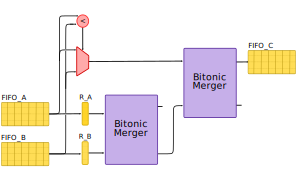
\includegraphics[width=10cm]{../figures/merger}
\end{center}
\caption{The design of a Hardware Merger as described in \cite{fccm18}.}
\end{figure}

\textit{Mergers} are hardware devices that take as input two sorted arrays, one element per cycle, and merge them so that the output list is sorted. Their design and functionality is explained in detail in the Implementation Section. These Mergers are then laid out as nodes in complete binary trees, called Merge Trees, whose analysis is the main topic of this paper. Merge Trees can be used to sort arrays by recursively merging elements of the array, as in the Merge Sort algorithm. On each recursive step, all elements of the input array are merged through the Merge Tree, thereby creating bigger and bigger sorted subsequences of the array until the array is fully sorted. We call each recursive step a \textit{stage} of the sorting process.

% \textcolor{blue}{\textbf{[EXPLAIN THE BASIC TRADE-OFF THAT THE MODEL EXPLORES]}}

Merge Trees are uniquely defined by their throughput and number of leaves. The throughput of a Merge Tree is the number of merged elements it outputs per cycle (we call this value $P$). The number of leaves of a Merge Tree is the number of leaf Merger nodes when viewing the Merge Tree as a complete binary tree (we call this value L). Previous work has not examined all possible combinations of $P$ and $L$, focusing mainly on $P = L$. We expanded the analysis of Merge Trees to any synthesizable combination of $P$ and $L$.

\begin{figure}[H]
\begin{center}
\includegraphics[width=6cm]{../figures/merger_tree}
\end{center}
\caption{Example architecture of a Merge Tree with throughput $P=4$ and number of leaves $L=8$.}
\label{example_P4_L8}
\end{figure}
\begin{figure}[p]
\begin{center}
\includegraphics[width=10cm]{../figures/merger_tree_bigger}
\end{center}
\caption{Example architecture of a Merge Tree with throughput $P=4$ and number of leaves $L=16$.}
\label{example_P4_L16}.
\end{figure}

 For example, for the Merge Tree with throughput of 8 elements per cycle and 16 leaves, we would use an 8-Merger at the root (depth 1), two 4-Mergers at depth 2, four 2-Mergers at depth 3, eight 1-Mergers at depth 4, and 16 1-Mergers at depth 5. An example of a throughput $P=4$ and number of leaves $L=16$ tree is in Figure~\ref{example_P4_L16}. An example of a throughput $P=4$ and number of leaves $L=8$ tree is in Figure~\ref{example_P4_L8}. When a $P$-Merger is connected as a child of a $2P$-Merger, we use a $P$-Coupler between them, which concatenates two consecutive outputs of the $P$-Merger for input into the $2P$-Merger. This has also been done in \cite{fccm17}. In our implementation, we may also have 1-Mergers be children of 1-Mergers in which case no Couplers are necessary and we just use a FIFO at the child-parent connection.

As recognized in \cite{terabyte}, having more leaves ($L$) in the Merge Tree reduces the total number of stages required to sort an array, thereby reducing the total sorting time. On the other hand, using a Merge Tree with higher throughput ($P$) reduces the total sorting time directly, by reducing the execution time for each stage. As increasing either $P$ or $L$ requires on-chip resources, there is a natural trade-off between these two parameters, which our model examines in detail.

\subsection{Our Contribution}

% \textcolor{blue}{\textbf{[MODEL CONTRIBUTION]}}

In this paper we present a comprehensive model for optimizing the choice of \textit{Merge Tree Set} based on the resources available on the FPGA and the off-chip memory bandwidth. A Merge Tree Set is defined as a triple
$(C, P, L)$, where $C$ is the number of Merge Trees in the set, $P$ is the throughput of one Tree, and L is the number of
leaves of one Tree. Even though it may be beneficial to use different Merge Trees, we restrict our search space to having $C$ equal Merge Trees as this simplifies optimization and off-chip read/write behavior.

% \textcolor{blue}{\textbf{[GREATER SEARCH SPACE CONTRIBUTION]}}

We decouple the Merge Tree throughput and number of leaves, thereby drastically increasing the optimization space. We also are also the first to implement a 1-Merger, which outputs only one element per cycle. The 1-Merger further increases to number of possible Merge Trees as the 1-Merger has a very small area, and thus can be used to build Merge Trees with a greater number of leaves. Note that the limited throughput of 1-Mergers is not a concern, as they either feed into other 1-Mergers or 2-Mergers, both of whose bandwidths will be saturated by having two 1-Mergers feeding into the input ports.

% \textcolor{blue}{\textbf{[DRAM ACCESS PATTERN CONTRIBUTION]}}

The other challenge that hasn’t been thoroughly addressed in previous work is the DRAM access pattern required by bigger Merge Trees. For Trees with many leaves, the DRAM access pattern has to be adequately implemented so that the accesses are predictable and sequential, while still being able to feed data into all of the leaves fast enough so that none of the leaves becomes starved. We address this issue in the implementation section.

% \textcolor{red}{\textbf{[STATE-OF-THE-ART END-TO-END SYSTEM CONTRIBUTION. First end-to-end system aside from Terabyte]}}

We ran cycle-accurate simulations to demonstrate that our end-to-end sorting system is state-of-the-art in terms of total runtime on FPGAs. Our model outperforms the implementation in \cite{terabyte} (the only other end-to-end sorting system on FPGAs) by 3.1x on identical hardware.

% \textcolor{blue}{\textbf{[FAST RESET CONTRIBUTION]}}

We implement controls that expand on the idea of \textit{Global Reset Signal Elimination} introduced in \cite{fccm18} by implementing a \textit{Fast Reset} procedure. This approach eliminates the \textit{setup time} required by Global Reset Signal Elimination and imposes minimal overheads. Most importantly it does not stall the datapath between different runs.
\section{Model}
\begin{wrapfigure}{r}{0.5\linewidth}
\includegraphics[width=7cm]{../figures/heatmap_performance}
\caption{Logarithmic heatmap of Performance ($P\log 2L$) as a function of the tree throughput ($P$) and number of leaves ($L$). Notice that Performance grows faster with the Merge Tree throughput ($P$) than with the number of leaves ($L$).}
\label{heatmap}
\end{wrapfigure}
Our model optimizes the choice and number of merger trees given the number of Look-Up Tables (LUTs) available and the off-chip memory bandwidth. Our goal is to optimize total sorting time. With $C$ merger trees running at frequency $f$, each of which has throughput $P$ elements per cycle and $L$ leaves, the total sorting time in seconds for 32-bit records can be approximated as follows:
\begin{equation}
\textrm{Total Sorting Time} = K\frac{N \log N/C}{f\cdot [CP \log 2L]},
\end{equation}
where $N$ is the total number of elements in the input array and $K$ is some universal constant. This equation holds because the total number of stages will be $\log_{2L}(N/C) = \frac{\log N/C}{\log 2L}$, and for each stage we process $N$ elements at a throughput of $f \cdot \min \{CP, OCMB\}$. For convenience, we can define a \textit{performance} metric for a set of C Merge Tree with throughput P and L leaves with
\begin{equation}
\textrm{Performance} = CP \log 2L.
\end{equation}



The logarithmic heatmap of some Merge Trees (defined by their $P$ and $L$ values) are given in Figure~\ref{heatmap}


One can use this Performance metric to quickly compare the effectiveness of different sets of merge trees. For example,
we can answer the following question: Which merge tree configuration is better:
\begin{itemize}[noitemsep,topsep=0pt,parsep=0pt,partopsep=0pt]
\item A single Merge Tree ($C_1 = 1$) with $P_1 = 8$, $L_1 = 4$, or
\item Three Merge Trees ($C_2 = 3$) with $P_2 = 4$, $L_2 = 4$?
\end{itemize}

We have $\textrm{Performance}_1 = 24$ and $\textrm{Performance}_1 = 36$, thus we can conclude the latter configuration will be about 50\% faster than the former configuration.

\subsection{Search Space Optimization}
\begin{wrapfigure}{r}{0.5\linewidth}
\includegraphics[width=7cm]{../figures/area}
\caption{Number of LUTs required by different Merge Trees: throughput ($P$) and number of leaves ($L$). This data is based on Vivado synthesis results.}
\label{luts}
\end{wrapfigure}
Aside from being able to predict the performance of Merge Trees, it is also important to consider the off-chip memory bandwidth and the area available on the FPGA. Then we can compare the Total Sorting Time of all Merge Trees that can be fit on the FPGA and choose the optimal one.


Figure~\ref{luts} shows the LUT utilization of a wide range of Merge Trees. We use these results to verify our area model. We approximate the resource utilization of a Merge Tree by adding up the resource utilization of its \textit{Building-Block Elements}. The Building-Block Elements are the Mergers (tree nodes) and Couplers that are used to build up any merge tree. The resource utilization of the Building-Block Elements we implemented is given in Table~\ref{tab:building_blocks}. Since using higher throughput Mergers requires superlinear area, it may be tempting to think that using multiple Merge Trees with low throughput is always better than using a single high-throughput Merge Tree. This, however, is usually not the case. This is because using two Merge Trees with lower throughput requires that we replicate all the Mergers used in the Trees. Of course, the root Merger and its children will require less than half the area of the root of the original double-throughput Tree, but the higher depth Mergers (root's great-grandchildren) would also have to be replicated. Since in most Trees the leaf nodes and other higher depth Mergers are usually 1-Mergers, we will not be able to use a smaller Merger if we decide to use two smaller throughput Trees instead of one high throughput Tree. Thus, for higher depth Mergers, the total area used by the two Trees will be double that of the original single high throughput Tree. Since most of the Mergers in a Tree are 1-Mergers, the total increase in area due to doubling the 1-Mergers will be far higher than the decrease due to using smaller Mergers close to the root.


If a different Merger or Coupler implementation is used, the resource utilizations of Building-Block Elements should be adapted to these implementations before our model is applied. Thus, our area (LUTs) model can be written down as:
\begin{align}
\textrm{Area}(P,L) &= \max \{0, 2L-P\}(M_1+F) - 1_{\{ 2L-P>0\}}PF \\
							 &+\sum_{n=0}^{\infty} 1_{\left\{\left\lfloor \frac{P}{2^n} \right\rfloor < L\right\}}\left\lfloor \frac{P}{2^n}\right\rfloor (M_{2^n} + 2C_{2^{n}}) +\sum_{n=0}^{\infty} 1_{\left\{\left\lfloor \frac{P}{2^n} \right\rfloor = L\right\}}\left\lfloor \frac{P}{2^n}\right\rfloor M_{2^n},
\end{align}
with $F$ being the number of LUTs used by a 32-bit FIFO (in our case, $50$ LUTs), $C_n$ being the number of LUTs used by an $n$-element Coupler, and $M_n$ being the number of LUTs used by an $n$-element Merger. Also, $1_{\{P\}}$ is the indicator function, equal to $1$ if the predicate $P$ is true, and $0$ otherwise. Although the equation seems daunting, it is just the sum of all the Building Block Elements (Mergers, FIFOs, and Couplers) required to construct a $(P, L)$ Merge Tree.

The accuracy of the area model is listed in~\ref{tab:results}.

\begin{table}[H]
\centering
\begin{tabular}{|c|c|c|c|c|}
\hline
\textbf{\textit{P}} &\textbf{\textit{L}}  &\textbf{LUTs}  & \textbf{Predicted} & \textbf{Error}  \\
\hline
1 &2  &978  &1,020  &4.1\%  \\
\hline
1 &4  &2,346  &2,380  &1.4\%  \\
\hline
1 &8  &5,107  &5,100  &  0.1\% \\
\hline
1 &16  &10,530  &10,540  &  0.1\% \\
\hline
1 &32  &21,420  &21,420  &  0.0\% \\
\hline
1 &64  &43,224  &43,180  &  0.1\%  \\
\hline
1 &128  &87,365  &86,700  &  0.8\%  \\
\hline
\hline
2 &2  &1,225  &1,486  &  \textcolor{red}{\textbf{17.5\%}} \\
\hline
2 &4  & 2,890 &2,846  &  1.5\% \\
\hline
2 &8  &5,618  &5,566  &  0.9\% \\
\hline
2 &16  &11,025  &11,006  & 0.2\% \\
\hline
2 &32  &21,875  &21,886  &  0.1\% \\
\hline
2 &64  &43,765  &43,646 &  0.3\% \\
\hline
2 &128  &86,702  &87,166  &  0.6\% \\
\hline
\hline
4 &2  &3,384  &3,345  & 1.1\%  \\
\hline
4 &4  &5,139  &5,073  & 1.3\% \\
\hline
4 &8  &7,879  &7,793  & 1.1\% \\
\hline
4 &16  &13,394  &13,233  & 1.2\% \\
\hline
4 &32  &24,105  &24,133  &  0.12\% \\
\hline
4 &64  &45,763  &45,873  &  0.2\% \\
\hline
4 &128  &89,011  &89,393  &  0.4\% \\
\hline
\end{tabular}
\quad\quad
\begin{tabular}{|c|c|c|c|c|}
\hline
\textbf{\textit{P}} &\textbf{\textit{L}}  &\textbf{LUTs}  & \textbf{Predicted} & \textbf{Error}  \\
\hline
8 &2  &7,912  &7,790  & 1.6\% \\
\hline
8 &4  &11,527  &11,370  & 0.2\% \\
\hline
8 &8  &15,068  &14,826  & 1.6\% \\
\hline
8 &16  &20,308  &20,266  & 0.2\% \\
\hline
8 &32  &31,152  &31,146  & 0.0\% \\
\hline
8 &64  &52,978  &52,906  & 0.1\% \\
\hline
8 &128  &96,262  &96,426  & 0.2\% \\
\hline
\hline
16 &2  &17,875  &17,834  & 0.2\% \\
\hline
16 &4  & 26,050 &26,174  & 0.5\% \\
\hline
16 &8  &33,669  & 33,334 & 1.0\% \\
\hline
16 &16  &40,249  &40,246  & 0.0\% \\
\hline
16 &32  &51,079  &51,126  & 0.1\% \\
\hline
16 &64  &73,275  &72,886  & 0.5\% \\
\hline
16 &128  &115,325  &116,406  & 0.9\% \\
\hline
\hline
32 &2  &39,761  &40,011 & 0.6\% \\
\hline
32 &4  &58,483   &58,679  & 0.3\% \\
\hline
32 &8  &75,165  &75,359  & 0.3\% \\
\hline
32 &16  &89,490  &89,679  & 0.21\% \\
\hline
32 &32  &103,600  &103,503  & 0.1\% \\
\hline
32 &64  &\textcolor{red}{\textbf{-}} &125,263  & \textcolor{red}{\textbf{-}} \\
\hline
32 &128  &169,724   &168,783  & 0.6\% \\
\hline
\end{tabular}
\caption{The accuracy of our area model compared with our experimental results.}
\label{tab:results}
\end{table}

\begin{table}[]
\centering
\begin{tabular}{|c|c|}
\hline
\textbf{Element} &\textbf{LUTs}  \\
\hline
1-Merger &300  \\
\hline
2-Merger &622 \\
\hline
4-Merger &1,555 \\
\hline
8-Merger &3,620 \\
\hline
16-Merger &8,500 \\
\hline
32-Merger &18,853 \\
\hline
\end{tabular}
\quad\quad
\begin{tabular}{|c|c|}
\hline
\textbf{Element} &\textbf{LUTs}  \\
\hline
32-bit FIFO &50 \\
\hline
1-Coupler &142 \\
\hline
2-Coupler &273 \\
\hline
4-Coupler &530 \\
\hline
8-Coupler &1,047 \\
\hline
16-Coupler &2,079 \\
\hline
\end{tabular}
\caption{LUT utilization of Building-Block Elements}
\label{tab:building_blocks}
\end{table}



Now, we restrict our search space for the optimal Merge Tree Set by considering only those sets that can be synthesized with the resources available on the FPGA. Figure~\ref{heatmap_area_curve} show the area cut-off for $200,000$ LUTs. Figure~\ref{shaded_area} has all the Merge Trees which require less than $200,000$ LUTs shaded in green.

\begin{figure}[H]
\begin{subfigure}{.5\textwidth}
\includegraphics[width=.9\textwidth]{../figures/heatmap_performance_area_high}
\caption{The Performance heatmap with the area curve. The Merge Trees whose centers of their respective cells are under the curve require less than $200,000$ LUTs.}
\label{heatmap_area_curve}
\end{subfigure} \quad
\begin{subfigure}{.5\textwidth}
\includegraphics[width=.9\textwidth]{../figures/heatmap_performance_single_shaded}
\caption{The logarithmic Performance heatmap with the Merge Trees that fit on $200,000$ LUTs shaded in green.}
\label{shaded_area}
\end{subfigure}
\end{figure}

Our model uses the off-chip memory bandwidth (OCMB) to ensure that the Merge Tree Set throughput is not unnecessarily high. For example, if the off-chip memory bandwidth is 10 GB/s, the effective throughput of, say, 2 Merge Trees
with P = 8 is not $2\cdot 8 = 16 GB/s$, but $\min\{2 \cdot 8, 10\} = 10 GB/s$, as the off-chip memory bandwidth will be a bottleneck to the throughput of the FPGA-CPU system. Figure~\ref{throughput_cutoff} illustrates the off-chip memory bandwidth cut-off; all Merge Trees to the right of the cut-off (shaded in red) have unnecessarily high throughput, i.e. the Merge Tree to the immediate left of the bandwidth cut-off will have the same performance as all the Merge Trees to the right of it, but will also require less area, thereby making all Merge Trees to the right of the bandwidth cut-off obsolete.

With all this in mind, we can derive an optimization target as

\begin{equation}
\textrm{Total Sorting Time} = K\frac{N \log N/C}{f\cdot \min\{CP, OCMB\} \log 2L},
\end{equation}
where our search space is limited to those Merge Tree Sets that can be mapped to the provided FPGA:
\begin{equation}
C \cdot \textrm{Area}(P,L) < \textrm{LUTs},
\end{equation}
where LUTs is the number of LUTs available to the FPGA. Depending on the implementation frequency we wish to achieve, the total number of available LUTs might have to be reduced artificially in order to be certain the design will be able to meet timing constraints. As an example, we used a Xilinx Virtex UtraScale+ FPGA VCU1252 which provides $1,182,240$ LUTs, yet we were only able to meet our $250$ MHz timing constraint with designed using under $130,000$ LUTs. Thus, we need a \textit{correction factor} $\eta$:
\begin{equation}
C \cdot \textrm{Area}(P,L) < \eta \cdot \textrm{LUTs},
\end{equation}



Our experimental results with the Vivado Synthesis tool suggest that the number of LUTs required by a model will be the resource bottleneck for Merge Trees on modern FPGAs. Thus, we do not model or worry about other on-chip resources like Block RAM (BRAM) or the total register (FF) usage.



Figure~\ref{four_things} gives the area cut-off and logarithmic heatmaps for using multiple Merge Trees of throughput $P$ and number of leaves $L$. Obviously, using more Merge Trees (greater Merge Tree Count, or $C$) requires more area. Thus, if we want to use mutliple Merge Trees, we cannot use Trees with as large a $P$ and $L$ value. However, our Performance on the heatmap will also grow linearly with the Merge Tree Count, given that $\textrm{Performance} = CP\log 2L$. (Notice that the same $P$ and $L$ values have brighter (higher) Performance values when we use more of the same tree) It is important to note that using more the Merge Tree Set throughput scales linearly with the Merge Tree Count ($C$), thus we must pay attention to not exceed the off-chip memory bandwidth when using multiple Merge Trees. Figure~\ref{four_things_four} gives cut-offs for different on-chip LUT counts.

As an example, the bottom-left heatmap tells us we can implement three ($C=3$) Merge Trees with throughput $P=2^5 = 32$ elements per cycle and $L=2^5=32$ leaves (the center of the $(5, 5)$ block is within the area cut-off) with a combined performance of about $2^9$. Conversely, the bottom-right heatmap tells us that we cannot implement four ($C=4$) such Merge Trees.

\begin{figure}[H]
\centering
\includegraphics[width=9cm]{../figures/heatmap_performance_throughput}
\caption{The logarithmic Performance heatmap with a throughput cut-off. In this example, the \textit{off-chip memory bandwidth} is limited to at most $2^4 = 16$ elements per cycle. Any Merge Trees that have throughput higher than this value will not give better sorting performance, as the throughput will be limited by the off-chip memory bandwidth.}
\label{throughput_cutoff}
\end{figure}
\newpage

\begin{figure}[H]
\begin{center}
\includegraphics[width=10cm]{../figures/heatmap_performance_limit_1}
\end{center}
\caption{The Performance heatmap for different Merge Tree Set sizes with the area cut-off. These graphs show which Merge Tree Sets can be implemented on $200,000$ LUTs.}
\label{four_things}
\end{figure}

\begin{figure}[H]
\begin{center}
\includegraphics[width=10cm]{../figures/heatmap_performance_limit_4}
\end{center}
\caption{The Performance heatmap similar to the one in Figure~\ref{four_things}, with area cut-offs for $100,000$ (green), $200,000$ (purple), $300,000$ (blue), $400,000$ (black), $500,000$ (pink).}
\label{four_things_four}
\end{figure}

\subsection{Data Skew}

% \textcolor{orange}{\textbf{[ADDRESS INPUT RATE MISSMATCH ISSUES]}}

If the input data for the leaves is not balanced (i.e., either one leaf has many more inputs than others, or has input data in a different range than other leaves), the Merge Tree might not work at its optimal throughput $P$. This is because a Merger node must stall whenever data is not available for one of its input FIFOs. One of the input FIFOs may become empty whenever the Merger consumes more data from one input than from the other, which is caused by unbalanced inputs. This issue has be reported in\cite{fccm18}, where the authors report the active rate to be 97\%. 

We believe probabilistic justification can be provided that will show that for uniformly random input data data skew will not present a problem on any tree.

\subsection{Model predictions}

% \textcolor{blue}{\textbf{[REPORT THE PREDICTED OPTIMAL MERGE TREE SET FOR DIFFERENT OCMB, LUT VALUES]}}

We give the model predictions based on the model described above in Table~\ref{tab:results_total}.
\begin{table}[H]
\centering
\begin{tabular}{|c|c|c|c|c|c|c|c|}
\hline
\textbf{Area$\backslash$OCMB} &1 [GB/s] &2 [GB/s] &4 [GB/s] &8 [GB/s] &16 [GB/s] &32 [GB/s] &64 [GB/s] \\
\hline
50,000 &(1, 1, 64)  &(1, 2, 64)  &(1,4,64)  &(1,8,32) &(1,16,16) &(3, 8, 8) &(32, 2, 2) \\
\hline
75,000 &(1, 1, 64)  &(1, 2, 64)  &(1,4,64) &(1,8,64) &(1,16,64) &(2, 16, 8) &(14, 4, 4) \\
\hline
100,000 &(1, 1, 128)  &(1, 2, 128)  &(1,4,128)  &(1,8,128) &(1,16,64) &(1, 32, 16) &(6, 8, 8)\\
\hline
130,000 &(1, 1, 128)  &(1, 2, 128)  &(1,4,128)  &(1,8,128) &(1,16,128) &(1, 32, 64) &(8, 8, 8) \\
\hline
150,000 &(1, 1, 128)  &(1, 2, 128)  &(1,4,128)  &(1,8,128) &(1,16,128) &(1, 32, 64) &(7, 8, 16) \\
\hline
200,000 &(1, 1, 256)  &(1, 2, 256)  &(1,4,256) &(1,8,256) &(1,16,128) &(1, 32, 128) &(2, 32, 16)\\
\hline
\end{tabular}
\caption{Optimal Merge Tree Sets $(C, P, L)$ with $C$ the number of Merge Trees in the set, $P$ the Merge Tree throughput, $L$ the number of leaves of the Merge Tree.}
\label{tab:results_total}
\end{table}
\begin{table}[H]
\centering
\begin{tabular}{|c|c|c|c|c|c|c|c|}
\hline
\textbf{Area$\backslash$OCMB} &1 [GB/s] &2 [GB/s] &4 [GB/s] &8 [GB/s] &16 [GB/s] &32 [GB/s] &64 [GB/s] \\
\hline
50,000 &47.60s  &23.80s  &11.90s  &6.94s &4.16s &3.31s &2.21s \\
\hline
75,000 &47.60s  &23.80s  &11.90s &5.95s &2.96s &2.52s &1.76s \\
\hline
100,000 &41.60s &20.83s  &10.41s  &5.20s &2.96s &2.08s &1.60s \\
\hline
130,000 &41.60s  &20.83s  &10.41s  &5.20s &2.60s &1.48s &1.18s \\
\hline
150,000 &41.60s  &20.83s  &10.41s  &5.20s &2.60s &1.48s &1.09s \\
\hline
200,000 &37.00s  &20.83s  &9.26s &4.63s &2.60s &1.30s &1.01s\\
\hline
\end{tabular}
\caption{The predicted total sorting time of the Optimal Merge Tree Sets $(C, P, L)$ specified in Table~\ref{tab:results_total} on $10$GB of 32-bit integer arrays. Cycle-accurate simulations demonstrate that the end-to-end system would be at most 10\% slower than the times listed here.}
\label{tab:results_total_2}
\end{table}
\section{Implementation}

Our design implementation is available on Github \cite{repo_link}. We have implemented our designs using Verilog. The DRAM-FPGA-CPU interface is implemented using SDAccel, with the CPU host code written in C++ using OpenCL. The on-chip memory interface is written in Verilog.

We first describe the Hardware Merger designed in ~\cite{fccm18} and our adaptations to that design. Then we explain how we build Merge Trees out of Mergers for any $P$ and $L$ value. Finally, we define the DRAM Access pattern.

The main differences between our design and the one employed in ~\cite{fccm18} is that we adapt the Global Reset approach with the \textit{Fast Reset} procedure, which minimizes the reset overhead between consecutive runs of the Mergers. Also, we forgo the use of pipelined CAS modules, as we do not require our Mergers to run at the frequencies specified in that paper. This means our designs have a smaller resource footprint, thereby allowing us to implement a wider range of Merge Trees.

\subsection{Hardware Mergers}

\begin{wrapfigure}{r}{0.5\linewidth}
\begin{center}
\includegraphics[width=4cm]{../figures/bitonic_merger}
\end{center}
\caption{The design of a 16-element bitonic merger, which is used in the 8-element Hardware Merger.}
\label{bitonic_merger}
\end{wrapfigure}

% \textcolor{blue}{\textbf{[SPECIFY THE BITONIC MERGER]}}

Figure~\ref{bitonic_merger} describes the Bitonic Merger, a basic building block of the Hardware Merger. Each horizontal line represents a 32-bit bus. The data flows left to right. The vertical arrows represent \textit{Compare-and-Swap} (CAS) units, which send the bigger of the two elements of the wire they connect in the direction of the arrow. The top and bottom half of inputs is assumed to be sorted and the bitonic merger then merges the top and bottom half in a pipelined fashion. The throughput of the Bitonic Merger in the Figure is thus 16 elements per cycle. A 16-element bitonic merger merges its input with a latency of $4$ clock cycles. During execution, each of the four pipelined areas in the design (CC 1, CC 2, CC 3, CC 4) hold and process a single 16 element array. In general, to merge two sorted $E$-record lists, $E+\log_2 E$ CAS units are required.

% \textcolor{blue}{\textbf{[SPECIFY NOMINAL BEHAVIOR OF HARDWARE MERGER]}}

Now we give the nominal behavior of the Hardware Merger, as presented in ~\cite{fccm18}. We consider a general $E$-record Merger. The registers $\textrm{R}_{\textrm{A}}$ and $\textrm{R}_{\textrm{B}}$ are used to store the dequeued elements from $\textrm{FIFO}_{\textrm{A}}$ and $\textrm{FIFO}_{\textrm{B}}$, respectively. The left Bitonic Merger has inputs $\textrm{R}_{\textrm{A}}$ and $\textrm{R}_{\textrm{B}}$. It outputs the largest $E$ records to the right bitonic merger. The smallest $E$ records output from the left Bitonic Merger are disregarded. The other inputs to the right merger are $E$ records from one of the FIFOs. The right Bitonic Merger outputs the smallest $E$ records, while the largest $E$ records are disregarded. 

\begin{figure}[H]
\begin{center}
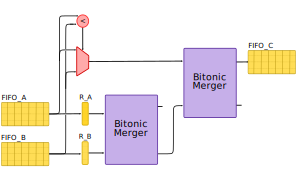
\includegraphics[width=6cm]{../figures/merger}
\end{center}
\caption{The design of a Hardware Merger as described in \cite{fccm18}.}
\end{figure}

At each clock cycle, whichever of $\textrm{FIFO}_{\textrm{A}}$ and $\textrm{FIFO}_{\textrm{B}}$ has the smallest minimal element at their top will be dequeued from. This dequeued element is then stored in either $\textrm{R}_{\textrm{A}}$ or $\textrm{R}_{\textrm{B}}$ (depending on if it came from $\textrm{FIFO}_{\textrm{A}}$ or $\textrm{FIFO}_{\textrm{B}}$ respectively) and is also forwarded as input to the right Bitonic Merger.

\subsubsection{Proof of Correctness}

% \textcolor{blue}{\textbf{[PROVE CORRECTNESS OF THE HARDWARE MERGER]}}

Let's justify the correctness of this design. Let $\textrm{R}_t$ be the set of $E$ records dequeued from from $\textrm{FIFO}_{\textrm{A}}$ or $\textrm{FIFO}_{\textrm{B}}$ at cycle $t$. We define the set of all dequeued records until cycle $t$ as $S_t = \bigcup_{i=1}^t r_i$. Let $f_t$ be the set of the biggest $E$ records output from the left Bitonic Merger. Let $S_t^A$ and $S_t^B$ be the sets of records dequeued from $\textrm{FIFO}_{\textrm{A}}$ and $\textrm{FIFO}_{\textrm{B}}$, respectively, from cycle 1 to cycle $t$. By definition, at cycle $t$, $\textrm{R}_{\textrm{A}}$ holds the largest $E$ records of $S_{t-1}^A$, and $\textrm{R}_{\textrm{B}}$ holds the largest $E$ records of $S_{t-1}^B$. Therefore, the largest $E$ records of $S_{t-1}^A \cup S_{t-1}^B$ are in $\textrm{R}_{\textrm{A}}$ and $\textrm{R}_{\textrm{B}}$ at cycle $t$.  This is because the local largest $E$ records in $\textrm{R}_{\textrm{A}}$ are the only candidates of $S_{t-1}^A$ for the global largest $E$ records of $S_{t-1}^A \cup S_{t-1}^B$, and the other local candidates of $S_{t-1}^B$ are exactly in $\textrm{R}_{\textrm{B}}$ as well. Thus, since $S_{t-1} = S_{t-1}^A \cup S_{t-1}^B$, then the output of the left Bitonic Merger at cycle $t$ ($f_t$) will be the largest $E$ records of $S_{t-1}$ (namely, the largest $E$ records of $\textrm{R}_{\textrm{A}} \cup R_{\textrm{B}}$). 

Thus, at cycle $t$, the right Bitonic Merger takes as its input $\textrm{R}_t$ and $f_t$, i.e. the smallest of the top of $\textrm{FIFO}_{\textrm{A}}$ and $\textrm{FIFO}_{\textrm{B}}$ and the largest $E$ records of $S_{t-1}$, respectively.By induction, we assume that the smallest $(t-2)E$ records of $S_{t-1}$ are already output at clock cycle $t-1$ and assume that these are indeed the $(t-2)E$ smallest records of the input array. We want to show that at clock cycle $t$, the output will be the $E$ smallest records of the input array that have not already been output. We already know exactly $E$ elements will be output and that these are by assumption bigger than all the elements that have already been output. We thus only need to show that the $E$ output elements will not be bigger than any other not yet output element. 

To show this, it is sufficient and necessary to prove that the $E$ smallest elements in $\textrm{R}_t \cup f_t$ are smaller than the smallest elements of both the tops of $\textrm{FIFO}_{\textrm{A}}$ and $\textrm{FIFO}_{\textrm{B}}$. Suppose without loss of generality, that $\textrm{R}_t \in S_t^A$, that is, that at clock cycle $t$ we dequeued from $\textrm{FIFO}_{\textrm{A}}$. Since the inputs to $\textrm{FIFO}_{\textrm{A}}$ and $\textrm{FIFO}_{\textrm{B}}$ are presorted by assumption, we know that the smallest element of the top of $\textrm{FIFO}_{\textrm{A}}$ (after dequeueing $\textrm{R}_t$) is bigger than any of the $E$ elements of $\textrm{R}_t$. Thus, it is also bigger than the smallest $E$ elements in $\textrm{R}_t \cup f_t$. 

We claim that the minimum element of the top of $\textrm{FIFO}_{\textrm{B}}$ is bigger than all the $E$ elements in $f_t$. Now, since $\textrm{FIFO}_{\textrm{B}}$ inputs are also presorted, we know that the minimum element of the top of $\textrm{FIFO}_{\textrm{B}}$ will be bigger than any element in $S_{t-1}^B$. First, since $\textrm{R}_t \in S_t^A$, we have by definition that the smallest element of the top of $\textrm{FIFO}_{\textrm{B}}$ is bigger than the minimum element of $\textrm{R}_t$ and also since the minimum element of $\textrm{R}_t$ is bigger than any element of $S_{t-1}^A$, we have that the minimum element of the top of $\textrm{FIFO}_{\textrm{B}}$ is bigger than any element of $S_{t-1}^A$ by transitivity. Further, the minimum of the top element of $\textrm{FIFO}_{\textrm{B}}$ is bigger than any element in $S_{t-1}^B$ as the input to $\textrm{FIFO}_{\textrm{B}}$ is sorted. Thus, since $f_t$ contains the biggest $E$ elements of $S_{t-1} = S_{t-1}^A \cup S_{t-1}^B$, and the minimum of the top element of $\textrm{FIFO}_{\textrm{B}}$ is bigger than any element of both $S_{t-1}^A$ and $S_{t-1}^B$, it is bigger than the biggest $E$ elements of $S_{t-1} = S_{t-1}^A \cup S_{t-1}^B$ and thus bigger than any element of $f_t$. Thus, the minimum element of the top of $\textrm{FIFO}_{\textrm{B}}$ is bigger than any of the $E$ smallest elements of $\textrm{R}_t \cup f_t$. This completes the correctness proof by induction.

\subsubsection{Fast Reset}

% \textcolor{blue}{\textbf{[SPECIFY IN DETAIL NOVELTY OF THE FAST RESET]}}

We first specify how the Mergers (and thus the Merge Trees) are reset between separate inputs (we call a set of inputs to the merge logic a \textit{run}). The idea of \textit{Global Reset Signal Elimination} is presented in \cite{fccm18}. We were, however, unable to find this feature in their implementation. Nonetheless, we were able to implement this idea and then improve it further.

As noted in \cite{fccm18}, to sort a large input dataset, we need to perform the merge operation recursively, going both through multiple runs and multiple stages. Thus, after the merge logic finishes merging the first set of lists, we have to make it ready to accept another two sequences. For example, we have to set all records in $\textrm{R}_{\textrm{A}}$ and $\textrm{R}_{\textrm{B}}$ of the merge network to zero.

A naive approach is to set all registers to zero using a global reset signal. However, this approach is not scalable, as it adds a large number of reset networks. To make our design completely scalable, we implement control only on the level of a single Merger. Thus, we must also reset locally instead of globally.

In \cite{fccm18}, the authors propose feeding dummy values (zeros) into the datapath until all the registers in the merge logic have been flooded with zero values. The time required to flush the tree with zeros is called the \textit{setup time}. Although this approach works, it may impose a big overhead, as at the beginning we transition between different runs rather quickly because the size of the sorted input chunks is small (see the Going Between Stages Section). Thus, the overhead of the setup time must be reduced to a minimum. We were able to adapt the control logic so that only a single dummy value (zero) must be fed between two different input lists to each of the input FIFOs without any additional requirements to stall the datapath between different runs (the new input can be fed in immediately after the single dummy input). This gives an overhead of $2L/P$ clock cycles for reseting the merge logic per run. Even for the first stage, which merger $8$-element sorted chunks, this will give an overhead of $(2L/P)/(16L/P) = 1/8 \sim 12.5\%$. For $2^n$-element sorted chunk inputs, the overhead will be $(2L/P)/(2^{n+1}L/P) = 2^{-n}$, or equivalently, the $k$-th stage will have a reset overhead of $(2L)^{1-k}/8$. We call this \textit{Fast Reset}.

\subsubsection{Hardware Merger Control Logic}

% \textcolor{blue}{\textbf{[SPECIFY THE CONTROL LOGIC]}}

Even though the nominal behavior of the Hardware Merger is fairly straightforward, there are many edge cases that need to be addressed. Namely, we must add control logic which operates as a Finite Statem Machine (FSM), together with a \textit{stall} signal. We must also implement the \textit{Fast Reset} procedure as described above.

The Finite State Machine transitions are given in Figure~\ref{state_transition}. The stall signal is defined as a wire and set as in Figure~\ref{stall_logic}. 

\begin{figure}
\begin{lstlisting}{H}
state <= (state == TOGGLE) ? (((~i_a_min_zero & ~i_b_min_zero) ? NOMINAL : TOGGLE)) :
          (state == DONE_A) ? ((i_b_min_zero ? TOGGLE : DONE_A)) :
          (state == DONE_B) ? ((i_a_min_zero ? TOGGLE : DONE_B)) :
		    (state == NOMINAL) ? (i_a_min_zero ? DONE_A : (i_b_min_zero ? DONE_B : NOMINAL));
\end{lstlisting}
\caption{The FSM State Transition Logic}
\label{state_transition}
\end{figure}

% \textcolor{blue}{\textbf{[SPECIFY IN DETAIL THE FSM CONTROL LOGIC OF THE MERGER]}}

The states and their purposes are:
\begin{itemize}[noitemsep,topsep=0pt,parsep=0pt,partopsep=0pt]
\item \textit{Toggle}. The Toggle state is active between while the dummy values between two different runs are being processed. In the Toggle state, elements are alternately popped from $\textrm{FIFO}_{\textrm{A}}$ and $\textrm{FIFO}_{\textrm{B}}$ until the dummy values are consumed.
\item \textit{Done A}. The Done A state is active when all the input from $\textrm{FIFO}_{\textrm{A}}$ has been consumed for the current run, but not from $\textrm{FIFO}_{\textrm{B}}$ (otherwise, Toggle would be active).
\item \textit{Done B}. The Done B state is active when all the input from $\textrm{FIFO}_{\textrm{B}}$ has been consumed for the current run, but not from $\textrm{FIFO}_{\textrm{A}}$ (otherwise, Toggle would be active).
\item \textit{Nominal}. The Nominal state is active when none of the other states are. This happens when we are in the middle of a run.
\end{itemize}

We now describe the state transitions in detail:
\begin{itemize}[noitemsep,topsep=0pt,parsep=0pt,partopsep=0pt]
\item \textit{From Nominal to Done A}. As stated above, the Nominal state is active as long as neither of $\textrm{FIFO}_{\textrm{A}}$ or $\textrm{FIFO}_{\textrm{B}}$ data has been consumed for this run. Thus, if the data is consumed for $\textrm{FIFO}_{\textrm{A}}$, the dummy value (zero) will be at the top of the FIFO and \verb!i_a_min_zero! will be high, thus the state will transition to Done A.
\item \textit{From Nominal to Done B}. Similarly to the above case, if the data is consumed for $\textrm{FIFO}_{\textrm{A}}$, the dummy value (zero) will be at the top of the FIFO and \verb!i_b_min_zero! will be high, thus the state will transition to Done B.
\item \textit{From Done A to Toggle}. In case the input from $\textrm{FIFO}_{\textrm{B}}$ is totally consumed for this run, \verb!i_b_min_zero! will become high. At this point both inputs from $\textrm{FIFO}_{\textrm{A}}$ and $\textrm{FIFO}_{\textrm{B}}$ will be consumed and thus we transition to the Toggle state.
\item \textit{From Done B to Toggle}. In case the input from $\textrm{FIFO}_{\textrm{A}}$ is totally consumed for this run, \verb!i_a_min_zero! will become high. At this point both inputs from $\textrm{FIFO}_{\textrm{A}}$ and $\textrm{FIFO}_{\textrm{B}}$ will be consumed and thus we transition to the Toggle state.
\item \textit{From Toggle to Nominal}. In case the dummy values (zeros) between runs have been consumed for both $\textrm{FIFO}_{\textrm{A}}$ and $\textrm{FIFO}_{\textrm{B}}$, we are ready to begin a new run and thus transition to the Nominal state. If at least one of $\textrm{FIFO}_{\textrm{A}}$ or $\textrm{FIFO}_{\textrm{B}}$ still has dummy values, we stay in the Toggle state and pop items from whichever FIFO still has dummy values.
\end{itemize}

\begin{figure}
\begin{lstlisting}{H}
assign stall = (i_fifo_out_full)   | ((state == NOMINAL) & (i_a_empty | i_b_empty)) 
                                     | (state == DONE_A & i_b_empty) 
                                     | (state == DONE_B & i_a_empty) 
                                     | (state == TOGGLE & (i_a_empty | ~i_a_min_zero) 
                                                          & (i_b_empty | ~i_b_min_zero) 
                                                          & (i_a_min_zero | i_b_min_zero));
\end{lstlisting}
\caption{The stall signal logic}
\label{stall_logic}
\end{figure}

Here are all of the possible reasons to stall a merger as implemented in Figure~\ref{stall_logic}:
\begin{itemize}[noitemsep,topsep=0pt,parsep=0pt,partopsep=0pt]
\item Output FIFO full.
\item One of the FIFOs goes empty during the run.
\item $\textrm{FIFO}_{\textrm{B}}$ goes empty during Done A.
\item $\textrm{FIFO}_{\textrm{A}}$ goes empty during Done B.
\item During the Toggle state, if one of the FIFOs is empty, and the other FIFO does not have any remaining dummy values to consume.
\item During the Toggle state, if one of the FIFOs' dummy values has been consumed, but the other FIFO's dummy values have not been consumed. Note that if both of the FIFOs have their dummy values consumed, we need not stall, as the state will transition to Nominal in that clock cycle.
\end{itemize}

\begin{figure}
\begin{lstlisting}{H}
select_A <= (new_state == NOMINAL & i_a_lte_b) 
           | (new_state == DONE_B) 
           | (new_state == TOGGLE & i_a_min_zero & ~i_a_empty);
\end{lstlisting}
\caption{The select logic}
\label{select_logic}
\end{figure}

Finally, the \verb!select_A! signal sets whether the Merger pops from $\textrm{FIFO}_{\textrm{A}}$ to $\textrm{R}_{\textrm{A}}$ (happens when \\ \verb!select_A == 1!) or if it pops from $\textrm{FIFO}_{\textrm{B}}$ to $\textrm{R}_{\textrm{B}}$ (happens when \verb!select_A == 0!). The selector logic is specified in Figure~\ref{select_logic}. During Nominal operation, the signal's value depends only on the comparison of the minimal elements of the top of $\textrm{FIFO}_{\textrm{A}}$ and $\textrm{FIFO}_{\textrm{B}}$ (\verb!i_a_lte_b!, read \textit{input less-than-or-equal-to b}). If we are in the Done B state, there is no input to process from $\textrm{FIFO}_{\textrm{B}}$ and thus we keep \verb!select_A! asserted. Finally, if the state is Toggle we only assert \verb!select_A! if a dummy value is on top of $\textrm{FIFO}_{\textrm{A}}$ (\verb!i_a_min_zero!) and $\textrm{FIFO}_{\textrm{A}}$ is not empty. Note that the Merger will stall if $\textrm{FIFO}_{\textrm{A}}$ is empty or its top is non-zero and also $\textrm{FIFO}_{\textrm{B}}$ is empty or its top is non-zero.



\subsection{Merge Trees}

% \textcolor{blue}{\textbf{[EXPLAIN HOW MERGE TREES OF VARIOUS SIZES CAN BE BUILT]}}

Merge Trees are built by laying out Hardware Mergers in a complete binary tree. Previous work has focused on a very small subset of Merge Trees, only looking at those with $P=L$. In this section we give examples on how arbitrary trees can be constructed.

First, let's describe how to construct a $P=4$, $L=16$ Merge Tree (Figure~\ref{example_P4_L16}). Tree throughput is defined by the throughput of the root Merger. Thus, the root Merger has to be a $4$-Merger. The two child Mergers of the root Merger must be at least $2$-Mergers, as the two child Mergers must together meet the throughput requirements of the parent. Since $2$-Mergers have half the throughput of a $4$-Merger, having $2$-Mergers as the child of the root will suffice. Note that using $4$-Mergers as root children would not increase the throughput of the Merge Tree, as the throughput would be constrained by the $4$-Merger at the root. Thus, using $4$-Mergers as children of the root would only unnecessarily increase the Merge Tree area.

Since $2$-Mergers output $2$ element wide data and the $4$-Merger has $4$ element wide input ports, two consecutive outputs of the $2$-Merger must be put side-by-side on a $4$ element wide bus before being fed into the input of the $4$-Merger. This job is done by a Coupler. (specifically a $2$-Coupler). The coupler takes two of its consecutive inputs and outputs them on a $4$ element wide bus.

The argument applied to the choice of the root's children applies to the choice of the children of the $2$-Mergers as well. Thus, the children of the $2$-Mergers are $1$-Mergers, with a $1$-Coupler in between that transforms $1$ element wide outputs of $1$-Mergers to $2$ element wide inputs of the $2$-Merger.

For children of $1$-Mergers, we do not have any smaller Mergers to choose and thus we use $1$-Mergers. Since the output of a child $1$-Merger is $1$ element wide, and the input to the parent $1$-Merger is also $1$ element wide, no Coupler is required at the child-parent connection. We nonetheless put a FIFO at the child-parent connection to mitigate Data Skew and Round Robin Skip issues; namely the FIFOs can be viewed as buffers that mitigate issues that arise from a specific leaf-to-root path being used more than average for multiple clock cycles.

\subsection{DRAM Access Pattern and the Round Robin Skip}

% \textcolor{blue}{\textbf{[ISSUES WITH THE DEFAULT APPROACH]}}


The DRAM access pattern we employ is illustrated in Figure~\ref{DRAM}. Ideally, the $2L$ input FIFOs would be able to request sequential 32-bit inputs from the DRAM whenever the FIFO is not full. There are multiple issues with this approach. First, the FPGA-DRAM bus is 512 bits wide. If the FIFOs requested 32 elements at a time, the bus would be severely underutilized. Second, although the addresses that the input FIFOs read from individually are sequential, the accesses between multiple FIFOs will be interleaved, meaning that the data access pattern to the DRAM will not be sequential. Third, when using many Merge Trees or using big trees, using a single AXI protocol to distribute the data to the input FIFOs would require a high wire fan-out.



% \textcolor{blue}{\textbf{[OUR APPROACH AND ROUND ROBIN SKIP]}}

In our approach we resolve all of these issues without leaving any input FIFOs unsaturated. We do this by reading in 512 sequential bits that will be fed into the first input FIFO in the first clock cycle. This 512-bit wide input is stored in a 512-bit wide FIFO that sits in front of the 32-bit input FIFO. (Figure~\ref{DRAM}). For the next $20$ clock cycles we keep reading 512 bits to be fed into the first input FIFO. Thus, all of the $20$ consecutive reads are sequential as they all feed into the first FIFO. This feeds a $1KB$ batch of data into the $512$-bit FIFO, which is a sufficiently large batch of sequential reads for the DRAM to be close to its peak bandwidth (Xilinx recommends that the reads to DRAM be batched into $1-4KB$ sequential reads)[oops, cannot find reference]. For the next $20$ reads, we feed 512 bits per cycle into a 512 bit FIFO in front of the second input FIFO. This process continues in a Round Robin fashion, spending 20 clock cycles per input FIFO in order to batch reads into sequential chunks.
\begin{wrapfigure}{r}{0.5\linewidth}
\begin{center}
\includegraphics[width=7cm]{../figures/feed_data}
\end{center}
\caption{The data loading scheme.}
\label{DRAM}
\end{wrapfigure}
The input FIFOs are then fed into via a small Control circuit. This circuit feeds the top 32-bit element of the top of the 512-bit FIFO when the input FIFO is not full. Then, if the input FIFO is still not full, the circuit feeds the next 32-bit element of the top of the 512-bit FIFO. This continues until the whole 512 bits of the top of the 512-bit FIFO have been exhausted. At that point, the top of the 512-bit is popped and the process continues from the top 32 bits of the new top of the 512-bit FIFO.

The 512-bit FIFOs in front of the input FIFOs that feed the leaf Mergers are 32 elements deep. This means each 512 bit FIFO requires $512 \times 32 = 2KB$ of storage. When synthesized, Vivado will implement these FIFOs using on-chip Block RAM (BRAM). This means a Merge Tree Set will require $(4L)KB$ of BRAM storage. Thus with 200 leaves, our system requires only $1MB$ of BRAM storage, which is manageable on modern FPGAs.

What should we do if the 512-bit FIFO does not have 20 free slots when it is its turn? One approach is to stall the Round Robin process until enough space becomes available on the 512-bit FIFO. Unfortunately, this approach may lead the whole tree to deadlock. Thus, our approach is to skip any FIFO that does not have 20 free slots available for input. This is why we call the algorithm the \textit{Round Robin Skip}. One concern may be that the skipped 512-bit FIFO may become empty way before the Round Robin algorithm comes to feed it again. However, since the 512-bit FIFO does not have 20 available slots, it then must store at least $(32-20)512/32 = 192$ 32-bit elements. Since the 32-bit input FIFO consumes one 32-bit element per cycle at most, the 512-bit FIFO will not get starved for at least another 192 cycles. In fact, in expectation it will not get starved for another $192\cdot 2L$ cycles. As the round robin algorithm will circle back to feed the FIFO in at most $20\cdot 2L$ cycles (assuming all other 512-bit FIFOs need to be fed), we have probabilistic assurance that none of the input FIFOs will be starved for too long.

To address the issue of the high fanout of the input data, we use up to $8$ input AXI bus protocols, each of which feeds only $2L/8$ FIFOs. This also reduces the probability of the input FIFOs starving.

\subsection{Going Between Stages}


% \textcolor{blue}{\textbf{[SPECIFY HOW THE MERGE TREE TRANSITIONS BETWEEN STAGES]}}


As mentioned in the Introduction, Merge Trees can be used to sort arrays by recursively merging elements of the array, as in the Merge Sort algorithm. On each recursive step, all elements of the input array are merged through the Merge Tree, thereby creating bigger and bigger sorted subsequences of the array until the array is fully sorted. We call each recursive step a \textit{stage} of the sorting process.This raises a couple of practical concerns. 


First a couple of definition: We say that an array $(a_0, a_1, …, a_N)$ has \textit{k-element sorted chunks} if for any $n < N/k$ the subsequence $(a_{nk}, a_{nk+1}, a_{nk+2}, …, a_{nk + (n-1)}, a_{n(k+1)})$ is sorted. We also call 
\begin{equation*}
(a_{nk}, a_{nk+1}, a_{nk+2}, …, a_{nk + (n-1)}, a_{n(k+1)})
\end{equation*}
 the $n$-th k-element sorted chunk.


Each stage is divided into \textit{runs}. Each run of a Merge Tree merges $2L$ input lists. For example, if the input to the Merge Tree with $L=4$ is a list of 512 elements with $8$-element sorted chunks, there will be a total of $512/(8\cdot 2\cdot 4) = 8$ runs, each merging $2L = 2\cdot 4$ $8$-element chunks. Namely, the first run will merge the $0$th, $8$th, $16$th, $24$th, $32$nd, $40$th, $48$th, and $56$th $8$-element chunks. The second run will merge the $1$st, $9$th, $17$th, $25$th, $33$rd, $41$st, $49$th, and $57$th $8$-element chunks. The third run will merge the $2$nd, $10$th, $18$th, $26$th, $34$th, $42$nd, $50$th, and $58$th $8$-element chunks, \textit{etc.}

For our model, we assume the fed in data comes in with 8-element sorted chunks. Initially sorting the list into $8$-element chunks can either be done on the FPGA or on the CPU using SIMD instructions (note that sorting many $8$-element lists is something the CPU is very good at as for such small lists the memory bottleneck is not an issue).

% \textcolor{blue}{\textbf{[EXAMPLE: HOW TO SORT $2^{15}$ ELEMENTS]}}

\begin{table}[H]
\renewcommand{\arraystretch}{2}
\centering
\begin{tabular}{|c|c|c|c|c|}
\hline
\textbf{Stage} &\textbf{Output Chunk Size}  &\textbf{Runs}  & \textbf{Num. Chunks Out} & \textbf{$n$-th FIFO Input Range}  \\
\hline
1 &64 &512 &512 &$2^{12}n-2^{12}(n+1)$ \\
\hline 
2 &512 &64 &64 &$2^{12}n-2^{12}(n+1)$ \\
\hline 
3 &4096 &8 &8 &$2^{12}n-2^{12}(n+1)$ \\
\hline 
4 &32,768 &1 &1 &$2^{12}n-2^{12}(n+1)$ \\
\hline
\end{tabular}
\caption{Summary of the behavior of the different stages required to sort $2^{15}$ elements}
\label{tab:stages}
\end{table}

Let's give an example of the structure of stages and runs for sorting a $2^{15} = 32,768$ input list that is sorted into $8$-element chunks. Assume we are using a single $L=4$ Merge Tree. The discussion is summarized in Table~\ref{tab:stages}.

The first stage will sort a total of $2^{15-3}=2^{12}\quad$ $8$-element chunks into a total of $2^{12-3}=2^9\quad$ $8\cdot 8 = 64$-element chunks. This will require $2^{12}/(2L) = 2^{12-3} = 2^9$ runs. The first $32,768/(2L) = 2^{12}$ elements are fed into the first input FIFO. The next $2^{12}$ elements are fed into the second FIFO, \textit{etc}. 

The second stage will sort the $2^9$ $64$-element chunks into a total of $2^{9-3} = 2^6\quad$ $8\cdot 64 = 512$-element chunks. This stage will require $2^9/(2L) = 2^6$ runs. 

The third stage will sort the $2^6$ $512$-element chunks into a total of $2^{6-3}=2^3\quad$ $8 \cdot 64 = 4096$-element chunks. This stage will require $2^6/(2L) = 2^3$ runs. The first $2^{12}$ elements will again be fed into the first FIFO. The next $2^{12}$ elements will again be fed into the second FIFO (the indices of the elements fed into each input FIFO does not change between runs).

The fourth stage will sort the $2^3$ $4096$-element chunks into $2^{3-3} = 1$ $32,768$-element chunk. This stage will require $2^3/(2L) = 1$ run. At this point the input list is sorted.

% \textcolor{blue}{\textbf{[HOW TO FEED IN DATA WITH DUMMY VALUES AND FILTER AT OUTPUT]}}

As described in the Fast Reset section, different runs of a stage need to be separated by a single dummy element (zero) for the Merge Tree to reset it is dealing with different sets of inputs. No other signals are needed to reset the Merge Tree. Note that we cannot speak of a reset of the Merge Tree and that the reset actually happens at each Merger whenever the dummy value reaches it. Since there is no stalling between different runs, it usually happens that the root Merger is still outputing data from the previous run while the leaf Mergers are processing data from the new run and the dummy values that separate the two runs are somewhere in between the leaves and the root.

Thus, we not only assume that the input list is presorted into $8$-element sorted chunk, but that these chunks are also separated by dummy values (a single 32-bit zero element). The Merge Tree is implemented so that, at the output of a stage, different sorted chunks will be already separated by dummy values at the output. Thus, the output from one stage can be fed in as input to the next stage without any changes to the data. 

In practice, however, the output from a stage will have many redundant zeros. To improve performance, we filter the Tree output by removing duplicate zeros. Specifically, any subsequence of consecutive zeros of the output is truncated to a single 32-bit zero element. This reduces the performance overhead of processing the dummy values and also makes it easier to partition the output into disjoint subsequences to be fed into the next stage as discussed in the above paragraphs. 

Thus, we must modify the $n$-th FIFO Input Range column in Table~\ref{tab:stages}, so that the dummy values between sorted chunks fit into the range. (This column reports the indices of the input list elements that are fed in order to the $n$-th Input FIFO). Let's do this for the $2^{15}$ element input example above. The updated results are summarized in Table~\ref{tab:updated}. The details are below.

\begin{table}[H]
\renewcommand{\arraystretch}{2}
\centering
\begin{tabular}{|c|c|c|c|c|}
\hline
\textbf{Stage} &\textbf{Output Chunk Size}  &\textbf{Runs}  & \textbf{Num. Chunks Out} & \textbf{$n$-th FIFO Input Range}  \\
\hline
1 &64 &512 &512 &$(2^{12}+512)n-(2^{12}+512)(n+1)$ \\
\hline 
2 &512 &64 &64 &$(2^{12}+64)n-(2^{12}+64)(n+1)$ \\
\hline 
3 &4096 &8 &8 &$(2^{12}+8)n-(2^{12}+8)(n+1)$ \\
\hline 
4 &32,768 &1 &1 &$(2^{12}+1)n-(2^{12}+1)(n+1)$ \\
\hline
\end{tabular}
\caption{Summary of the behavior of the different stages required to sort $2^{15}$ elements}
\label{tab:updated}
\end{table}

For the first stage, there are a total of $2^{15}/8 = 2^{12}\quad$ $8$-element chunks. Each input FIFO receives $2^{12-3}=2^9$ of these chunks. Each chunk will be prepended with a dummy value (zero). Thus, each FIFO will receive an additional $2^9$ elements. Thus, the $n$-th FIFO Input range will now be $(2^{12}+2^9)n-(2^{12}+2^9)(n+1)$ for the first stage.

For the second stage, there are a total of $2^{12}/8 = 2^{9}\quad$ $64$-element chunks. Each input FIFO receives $2^{9-3}=2^6$ of these chunks. Thus, the $n$-th FIFO Input range will now be $(2^{12}+2^6)n-(2^{12}+2^6)(n+1)$ for the first stage, \textit{etc.}

In general, if the input list to a stage has $N$ chunks and the Merge Tree has $L$ leaves, the number of dummy values that have to be accounted for is $N/(2L)$. Thus, each input FIFO will get $N/(2L)^2$ of these dummy values. In general, assuming we start with $N\quad$ $8$-element sorted chunks, the $k$-th stage will have the input to each input FIFO be exactly $8N + N/(2L)^{k+1}$ elements. 

The overheads caused by inserting the dummy values into the datapath are reported in the Fast Reset section.

\section{Experimental Results}
We ran our experiments on the Xilinx Virtex UltraScale+ FPGA VCU1525 and use our own Merger and Coupler implementations that are based on the work in \cite{fccm18}. We also report results that we got from cycle-accurate simulations of our Verilog code. We choose to run our implementation at 250 MHz (versus 125 MHz in \cite{terabyte}). This frequency is also the frequency of the DRAM-FPGA bus. Our DRAM bus is 512 bits wide. We were able to synthesize Merge Trees for any combination of the following values of the throughput $P$ and number of leaves $L$:
\begin{align*}
L &= \{1,2,4,8,16,32,64,128\}, \\
P &= \{1,2,4,8,16,32\},
\end{align*}
except for $(P,L) = \{(32, 64), (32,128)\}$.

% \textcolor{blue}{\textbf{[REPORT AREA]}}

The predictions of the area model together with experimental results and relative errors of the predictions are listed in Table~\ref{tab:results}. We notice that all predictions are within $2\%$ of the actual area reported by Vivado Implementation, except for the Merge Tree with $(P, L) = (2, 2)$ in which our prediction overestimated the area by $17\%$. The Vivado Utilization tool reports that the $2$-Merger used by this tree has a significantly lower area (lower by $200$ LUTs) than the area utilization reported by the stand-alone $2$-Merger. We were unable to get to the cause of this issue.

The active rate and number of cycles required to perform each merging stage for an input of $2^{15}$ elements is listed in Table~\ref{tab:stages_cycles}.

\begin{table}[H]
\renewcommand{\arraystretch}{2}
\centering
\begin{tabular}{|c|c|c|c|c|}
\hline
\textbf{Stage} &\textbf{Output Chunk Size}  &\textbf{Measured Cycles}  & \textbf{Optimal Cycles} & \textbf{Active Rate}  \\
\hline
1 &64 &9,405 &7,629 &95\% \\
\hline 
2 &512 &8,537 &7,629  &95\% \\
\hline 
3 &4,096 &8,636 &7,629  &96\% \\
\hline 
4 &32,768 &8,650 &7,629  &87\% \\
\hline
\hline
Total &- &35,228 &30,517 &93\% \\
\hline
\end{tabular}
\caption{The optimal and measured number of cycles required for each of the $4$ stages required by the $(P,L)=(4,4)$ tree to sort $2^{15}$ elements. The optimal number of cycles reflects the number of cycles required to complete the stage if data skew, DRAM access latency issues, and dummy value overhead did not exist, that is, if the tree operated at $4 GB/s$. \textit{Active rate} specifies the ratio of measured and optimal performance.}
\label{tab:stages_cycles}
\end{table}

We have not yet been able to implement the DRAM access pattern as described in the DRAM Access Pattern and Round Robin Skip sections. We have only implemented an end-to-end solution for $(P, L) = (4, 4)$ and instead of using a single AXI Protocol, we use $8$ different AXI Protocols, each of which is responsible for a single 512-bit FIFO. This approach requires 10x the time predicted by our model. We conjecture that this performance hit is due to the different AXI Protocols competing for DRAM Access. This then makes the DRAM Controller switch between servicing the requests of different AXI Protocols. If this is the case, the actuall accesses to DRAM are neither sequential nor batched. To mitigate this issue, we plan to implement an end-to-end system as specified in the DRAM Access Pattern section.

\newpage
\begin{thebibliography}{9}

\bibitem{fccm17}
Susumu Mashimo, Thiem Van Chu, and Kenji Kise.
\textit{High-Performance Hardware Merge Sorter}.
IEEE 25th Annual International Symposium on Field-Programmable Custom Computing Machines, 2017.

\bibitem{fccm18}
Susumu Mashimo, Thiem Van Chu, and Kenji Kise.
\textit{A High-Performance and Cost-Effective Hardware Merge Sorter without Feedback Datapath}.
IEEE 26th Annual International Symposium on Field-Programmable Custom Computing Machines, 2018.

\bibitem{camb}
Wei Song, Dirk Koch, Mikel Luj{\'a}n, and Jim Garside.
\textit{Parallel Hardware Merge Sorter}
IEEE 25th Annual International Symposium on Field-Programmable Custom Computing Machines, 2016.

\bibitem{terabyte}
Sang-Woo Jun, Shuotao Xu, Arvind.
\textit{Terabyte Sort on FPGA-Accelerated Flash Storage}.
IEEE 25th Annual International Symposium on Field-Programmable Custom Computing Machines, 2017.

\bibitem{nyt_article}
John Markoff.
\textit{Smaller, Faster, Cheaper, Over: The Future of Computer Chips}.
New York Times, Sept. 26, 2015.

\bibitem{end_of_moore}
Elie Track, Nancy Forbes, and George Strawn.
\textit{The End of Moore's Law}.
Computing in Science \& Engineering, Vol. 19, Issue 2, Mar.-Apr. 2017.

\bibitem{mapreduce}
Jeffrey Dean and Sanjay Ghemawat.
\textit{MapReduce: Simplified Data Processing on Large Clusters}.
Communications of the ACM - 50th anniversary issueL 1958-2008, pp. 107-113.

\bibitem{microsoft_merge_join}
Goetz Graefe.
\textit{The Value of Merge-Join and Hash-Join in SQL Server}.
VLDB Proceedings of the 25th International Conference on Very Large Data Bases, 1999.

\bibitem{eth_merge_join}
Claude Barthels, Ingo M{\"u}ller, Timo Schneider, Gustavo Alonso, Torsten Hoefler.
\textit{Distributed Join Algorithms on Thousands of Cores}.
Proceedings of the VLDB Endowment, Vol. 5, Issue 5, Jan. 2017, pp 517-528.

\bibitem{joulesort}
Suzanne Rivoire, Mehul A. Shah, Parthasarathy Ranganathan, Christos Kozyrakis.
\textit{JouleSort: A Balanced Energy-Efficiency Benchmark}.
Proceedings of the 2007 ACM SIGMOID International Conference on Management of Data, pp. 365-276, 2007.

\bibitem{cloudsort}
Mehul A. Shah, Amiato, Chris Nyberg, Ordinal Technology Corp., Naga Govindaraju, Microsoft (Azure).
\textit{CloudSort: A Total-Cost of Ownership (TCO) Sort Benchmark}.

\bibitem{alphasort}
Chris Nyberg, Tom Barclay, Zarka Cvetanovic, Jim Gray, Dave Lomet.
\textit{AlphaSort: A Cache-Sensitive Parallel External Sort}. The International Journal on Very Large Data Bases, Vol. 4, Issue 4, October 1995.

\bibitem{tencent}
Jie Jiang, Lixiong Zheng, Junfeng Pu, Xiong Cheng, Chongqing Zhao, Mark R. Nutter, Jeremy D. Schaub.
\textit{Tencent Sort}.
Tencent Corporation, 2016.

\bibitem{nadsort}
Qian Wang, Rong Gu, Yihua Huang, Reynold Xin, Wei Wu, Jun Song, Junluan Xia.
\textit{NADSort}.
Nanjing University, Databricks Inc., Alibaba Group Inc., 2016.

\bibitem{ntosort}
Andreas Ebert.
\textit{NTOSort}.
Microsoft.

\bibitem{cache-friendly}
Hiroshi Inoue, Kenjiro Taura.
\textit{SIMD- and Cache-Friendly Algorithm for Sorting an Array of Structures}.
Proceedings of the 41st International Conference on Very Large Data Bases, Vol. 8, Issue 11, July 2015.

\bibitem{SIMD}
Jatin Chhugani, William Macy, Akram Baransi.
\textit{Efficient Implementation of Sorting on Multi-Core SIMD CPU Architecture}.
Proceedings of the International Conference on Very Large Data Bases, Vol. 1, Issue 2, July 2008.


\bibitem{radix}
Minsik Cho, Daniel Brand, Rajesh Bordawekar.
\textit{PARADIS: An Efficient Parallel Algorithm for In-Place Radix Sort}.
Proceedings of the 41st International Conference on Very Large Data Bases, Vol. 8, Issue 12, August 2015.

\bibitem{manycore}
Nadathur Satish, Mark Harris, Machael Garland.
\textit{Designing Efficient Sorting Algorithms for Manycore GPUs}
IEEE International Symposium on Parallel \& Distributed Processing, 2009.

\bibitem{gputera}
Naga K. Govindaraju, Jim Gray, Ritesh Kumar, Dinesh Manocha.
\textit{GPUTeraSort: High Performance Graphics Co-processor Sorting for Large Database Management}.
Proceedings of the 2006 ACM SIGMOID International Conference on Management of Data, 2006.

\bibitem{gpu_radix}
Duane Merrill, Andrew Grimshaw.
\textit{High Performance and Scalable Radix Sorting: A Case Study of Implementing Dynamic Parallelism for GPU Computing}.
Parallel Processing Letters, June 2011.

\bibitem{gpu_survey}
Dmitri I. Arkhipov, Di Wu, Keqin Li, Amelia C. Regan.
\textit{Sorting with GPUs: A Survey}.

\bibitem{farmahini}
Amin Farmahini-Farahani, Henry J. Duwe III, Michael J. Schulte, Katherine Compton.
\textit{Modular Design of High-Throughput, Low-Latency Sorting Units}.
IEEE Transactions on Computers, July 2013.

\bibitem{lhc}
Amin Farmahini-Farahani, Anthony Gregerson, Michael Schulte, Katherine Compton.
\textit{Modular High-Throughput and Low-Latency Sorting Units for FPGAs in the Large Hadron Collider}.
IEEE 9th Symposium on Application Specific Processors, 2011.

\bibitem{fpgasort}
Dirk Koch, Jim T{\o}rresen.
\textit{FPGASort: A High Performance Sorting Architecture Expoiting Run-time Reconfiguration on FPGAs for Large Problem Sorting.}
IEEE 24th Annual International Symposium on Field-Programmable Custom Computing Machines, 2016.

\bibitem{dbo}
Jared Casper, Kunle Olukotun.
\textit{Hardware Acceleration of Database Operations}
Proceedings of the ACM/SIGDA International Symposium on Field-programmable Gate Arrays, 2015.

\bibitem{unbalanced_fifo}
Rui Marcelino, Hor{\'a}cio C. Neto, Jo{\~a}o M. P. Cardoso, 
\textit{Unbalanced FIFO Sorting for FPGA-based Systems}.
IEEE International Conference on Electronics, Circuits, and Systems (ICECS), 2009.

\bibitem{network}
Rene Mueller, Jens Teubner, Gustavo Alonso.
\textit{Sorting Networks on FPGAs}.
The International Journal on Very Large Data Bases, Vol. 21, Issue 1, February 2012.

\bibitem{eth}
Marcela Zuluaga, Peter Milder, Markus P{\"u}schel.
\textit{Computer Generation of Streaming Networks}.
Design Automation Conference (DAC), 2012.

\bibitem{usc}
Ren Chen, Sruja Siriyal, Viktor Prasanna.
\textit{Energy and Memory Efficient Mapping of Bitonic Sorting on FPGA}.
Proceedings of the 2015 ACM/SIGDA International Symposium on Field-programmable Gate Arrays, 2015.

\bibitem{usc2}
Chi Zhang, Ren Chen, Viktor Prasanna.
\textit{High Throughput Large Scale Sorting on a CPU-FPGA Heterogeneous Platform}.

\bibitem{mit_merge_tree}
Kermin Fleming, Myron King, Man Cheuk Ng.
\textit{High-throughput Pipelined Mergesort}.
ACM/IEEE International Conference on Formal Methods and Models for Co-Design, 2008.

\bibitem{repo_link}
\url{https://github.com/n-samar/research_helpers}.

\end{thebibliography}
\end{document}
